\documentclass[12pt,fleqn]{article}\usepackage{../../common}
\begin{document}
Materyel Mekaniği - Hazırlık

Eksenel Yükleme (Uniaxial Loading)

Pek çok problemde kullanılan en temel deformasyon (yamulma, şekil değiştirme)
türü altta görülen tür yüklemedir. Bir demir, ya da plastik çubuk iki kuvvetle
boyu yönünde (tek bir eksende yani) iki tarafa doğru çekilir, bizim
ilgilendiğimiz çubukta seçilen herhangi bir noktanın nereye gittiği, yani o tek
eksendeki deformasyonun ne olduğu.

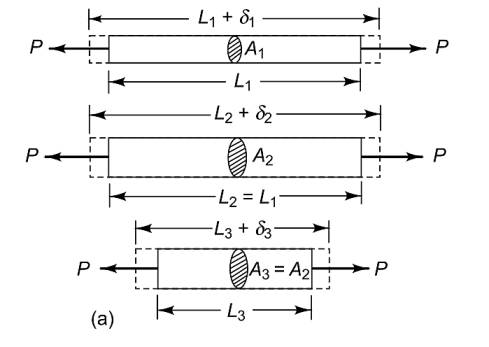
\includegraphics[width=20em]{phy_020_strs_00_01.jpg}

Diyelim ki üstteki her üç çubuk aynı maddeden yapılmış, farklı uzunlukları ve
kalınlıkları var, her çubuğa sıfırdan başlayarak belli seviyelerde $P$ kuvveti
ile yük uyguluyoruz, ve çubuğun uzunluk değişimi (elongation) $\delta$
değerinin, ki tek boyuttaki deformasyon budur, ne olduğuna bakıyoruz. Her 1,2,3
çubuğu için $P/A$ ve $\delta/L$ değerlerini grafiklersek çoğunlukla sonuç ya alt
soldaki gibi ya da sağdaki gibi çıkacaktır [1, sf. 76].

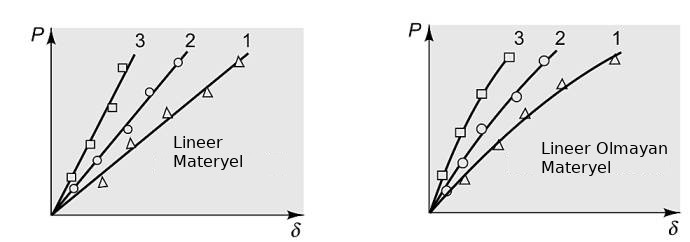
\includegraphics[width=20em]{phy_020_strs_00_02.jpg}

Eğer materyelin eksenel yük ve uzama ilişkisi lineer ise o zaman sonuç soldaki
resim gibi çıkar. Grafiğin eğimine elastiklik genliği (modulus of elasticity)
adı verilir ve çoğunlukla ona $E$ sembolü verilir. Formülsel olarak belirtirsek,

$$
E = \frac{P/A}{\delta / L}
\mlabel{1}
$$

$E$ formülüne Young'in Genliği (Young's Modulus) ismi de verilir. 

$\delta/L$ büyüklüğü mevcut büyüklüğe nazaran ne kadar uzama olduğunu gösteren
bir oran, mesela 200 cm için 2 cm büyüme var ise 2/200, bu bir tür yüzde hesabı
olarak görülebilir (ek olkarak yüz ile de çarpmak gerekir ama aşağı yukarı öyle).

Not: $P$ çoğunlukla basınç (pressure) için kullanılır ama burada kuvvet.

$P/A$'nin birimi kuvvet bölü birim alan olduğu ve $\delta / L$ birimsiz olduğu
için $E$'nin birimi de kuvvet bölü birim alan olacaktır. Daha ileride göreceğiz
ki $P/A$ bir alan $A$ üzerindeki ortalama {\em stres} değeridir, $\delta / L$
ise $L$ boyunca hissedilen {\em gerilme} değeridir (strain).

Yani $E$ birimi Newton bölü metrekare olacaktır, $N/m^2$ ya da Pascal, Pa terimi
kullanılabilir. Bazı tipik değerler demir ve çelik için $200\cdot 10^6$ kilo
Newton / $m^2$, aliminyum için $69 \cdot 10^6$ $kN / m^2$.

(1) formülünü düzenleyip tekrar yazarsak, 

$$
\delta = \frac{PL}{AE}
$$

Üstteki formül Hooke Kanunu'nun basit bir formudur aslında; bu isim Robert Hooke
bilimcisine atfendir, ki pek çok materyelin yük-deformasyon eğrisinin lineer
olduğunu keşfeden Hooke'tur. Bu arada materyelin eğrisi lineer ise bu durum
sarma yaylar (coiled springs) için de aynıdır. Kavramsal ve formülsel olarak
bir demir çubuğu yay olarak görsek mesela $10^3 mm^2$ genişliğinde ve
1 metre uzunluğunda, Hooke Kanunu

$$
F = k x
$$

ki $F$ kuvvet, $k$ yay sabiti ve $x$ uzama, mevcut semboller ile,

$$
P = k \delta
$$

$$
k = \frac{P}{\delta}
$$

$$
= \frac{P}{PL / AE} = \frac{1}{L / AE} = \frac{AE}{L} =
\frac{10^3 10^{-3} 205}{1} =
205 GN/m
$$

Demir Çubuk Gerilmesi

Daha önce gördüğümüz üzere bir normal gerilme $\epsilon$'nin baz tanımı

$$
\epsilon = \Delta L / L
\mlabel{2}
$$

ki $L$ mevcut uzunluk, $\Delta L$ uygulanan kuvvet sonucu elde edilen uzama [2].
Bu formülü ufak bir demir çubuk parçasının bükülmesine uygulayabilir miyiz
acaba? 

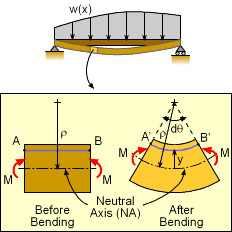
\includegraphics[width=15em]{phy_020_strs_00_03.jpg}

Üstteki resme göre formülleri yazabiliriz. Resimde alt solda bükülme öncesi,
sağda sonrası görülüyor, bükülme nötr eksenden $\rho$ uzaklığındaki bir nokta
etrafında ve $\ud\theta$ kadar. Bükülme öncesi $AB$ uzunluğu mesela görülen mavi
çizgi için $A'B'$ haline gelecek. Ama dikkat edersek nötr eksene yakın noktalar
daha az uzayacak, uzaklar daha fazla.. bu uzaklığı bir $y$ üzerinden temsil
edebiliriz. Bu uzaklığı hesaba katan bir gerilme formülü nasıl elde ederiz?

Nötr eksene $y$ uzaklığındaki $AB$ bükülme sonrası $A'B'$ oldu ise, bu durumu
(2) bazında belirtelim,

$$
\epsilon = \frac{A'B' - AB}{AB}
$$

Şimdi $A'B'$ hesabına gelelim. Dikkat edersek $A'B'$ ufak bir çember çevresi,
verili yarıçapı ve açı üzerinden bu çember çevresi hesaplanabilir, tüm daire
çevresi muhakkak $2 \pi r$, açısı bilinen ufak parçalar için $\pi \theta$,
burada açı $\theta$ tüm $2 \pi$'ye oranlı, radyan olarak. O zaman

$$
AB = \rho \ud \theta
$$

$A'B'$ için ufak dairenin yarıçapı değişir, nötr eksene $y$ kadar uzak isek,
$A'B'$ yarıçapı $\rho - y$, demek ki 

$$
A'B' = (\rho - y) \ud \theta
$$

Bunlari (2)'ye koyarsak,

$$
\epsilon = \frac{(\rho - y) \ud \theta - \rho \ud \theta}{\rho \ud\theta} =
\frac{\rho \ud\theta - y \ud\theta - \rho \ud\theta}{\rho \ud\theta} =
- \frac{y \ud\theta}{\rho \ud\theta}
$$

$$
= - \frac{y}{\rho}
$$



[devam edecek]

Kaynaklar

[1] Crandall, {\em An Introduction to the Mechanics of Solids}

[2] Gramoll, {\em Mechanics},
    \url{http://www.ecourses.ou.edu/cgi-bin/ebook.cgi?topic=me}

\end{document}


